\chapter{Marco Teórico}
\label{chap:marcoteorico}

% Estado del arte general de la temática de estudio. 
\section{Introducci\'on}

La estimaci\'on de errores en la determinaci\'on orbital en la base del procedimiento.(redactar mejor)\\
En un contexto ideal, de una Tierra esf\'erica, homog\'enea y sin rozamiento, los modelos f\'isicos que describen el movimiento de los objetos que orbitan la Tierra, nos permitir\'ian predecir con much\'isima precisi\'on las sitaciones de colisi\'on. Es decir, si conoci\'eramos muy bien la posici\'on de las naves y las condiciones del entorno, y pudi\'eramos modelarlo, podr\'iamos hacer predicciones futuras de las posciones y as\'i determinar si los objetos van a colisionar o no sin ambig\"uedad. Pero esa no es la realidad.\\
La Tierra no es perfectamente esf\'erica y mucho menos homog\'enea, y si bien es la principal influencia en las \'orbitas de las naves, existen otros cuerpos como la Luna, el Sol y los dem\'as planetas que tambi\'en ejercen fuerzas gravitatorias en mayor o menor medida.\\
Existen tambi\'en otras fuerzas, que resultan del entorno, como por ejemplo el frenado de la atm\'osfera para los objetos de \'orbitas LEO y la presi\'on de radiaci\'on solar que afecta principalmente a los sat\'elites con grandes paneles.\\

Todos estos condimentos, nos muestran que la determinaci\'on de las posiciones de los objetos que orbitan la Tierra, no es una tarea sencilla. Dependiendo de los distintos m\'etodos y modelos de determinaci\'on orbital con los que se cuentan, podremos saber con mejor o peor precisi\'on la posici\'on de los objetos.El estudio de riesgo de colisi\'on se basa en la capacidad de determinar y predecir las \'orbitas de los objetos involucrados en un acercamiento con la mayor precisi\'on posible.\\.
Esto implica un aspecto crucial en el estudio de las posibles colisiones, ya que cuando se pretenden hacer predicciones orbitales, debemos saber con qu\'e margen de error hemos calculado la sitauci\'on de acercamiento. Y es esta misma raz\'on la que explica por qu\'e en el c\'alculo de colisiones se habla de probabilidad de colisi\'on (PoC)\\

Mejorar estas estimaciones es fundamental, ya que en base a ellas se realizan o no maniobras, que, por un lado interfieren en los experimentos cient\'ificos que se llevan a cabo en las distintas plataformas, las maniobras son siempre operaciones delicadas, y en las misiones con astronautas a bordo (como por ejemplo la Estaci\'on Espacial Internacional (ISS)), una decisi\'on err\'onea pone en riesgo a la tripulaci\'on.\\

Por otra parte, distintos estudios realizados (... Foster ¿?), muestran que existen en varios m\'etodos actuales de c\'alculo de PoC, sobreestimaciones de los acercamientos y los riesgos, generando falsas alarmas que de no ser revisadas con minuciosidad conducen a decisiones de maniobras innecesarias. 

El epoca de la colisi\'on y la previsi\'on en los c\'alculos.(redactar)\\
La determinaci\'on orbital es m\'as f\'acil a posteriori.\\



\section{La Posici\'on de los objetos involucrados}

En nuestro planteo de riesgos por colisi\'on entre misiones operativas y desechos espaciales, existir\'an dos abordajes distintos del problema de la determinaci\'on de las posiciones, ya que cada uno de los objetos involucrados ofrece metodolog\'ias y modelos diferentes.

\subsection*{La posici\'on de la misi\'on operativa}
Con la misi\'on operativa tenemos contacto y comandado. En gral tiene un GPS o alg\'un otro instrumento de determinaci\'on de la posici\'on, con un cierto error asociado, que es conocido.({\bf{cu\'al?}})\\
A su vez CONAE tiene su modelo orbital de propagaci\'on y generaci\'on de predicci\'on (PREPHEM), y su propio modelo de ajuste (ORBEPHEM).\\

\subsection*{La posici\'on del desecho espacial}
El desecho espacial no tiene capacidades operativas, de manera que la \'unica manera de determinar su posici\'on es con redes de rastreo desde Tierra.\\
Caracter\'istica de las redes de rastreo. error asociado, que es conocido.({\bf{cu\'al?}})\\
S\'olo usa, rusia y la uni\'on europea cuentan con redes de rastreo. En particular Norad es la que disponibiliza en forma p\'ublica los datos en formato TLE.\\
Dado este contexto, las distintas agencias, que no cuentan con gran n\'umero de misiones operativas, suelen contratar/acordar este servicio. Y a\'un, con herramientas propias desarrolladas, lleva tiempo la validaci\'on de las mismas hasta lograr cierta autonom\'ia. No obstante, la tendencia es hacia un primer paso, que permita una caracterizaci\'on m\'as precisa de la situaci\'on de encuentro, sumando a la informaci\'on p\'ublica, m\'etodos de ajuste, datos propios de la misi\'on en riesgo y estimadores del riesgo como por ejemplo la \ac{PoC}.\\
Es en esa direcci\'on que planteamos este trabajo, a fin de ofrecer un prototipo que pueda ser implementado en paralelo a lo que ya se utiliza en CONAE, para ser probado y mejorado con la experiencia que sumen los encuentros que involucren a las misiones nacionales.\\
Describir:\\
\begin{itemize}
\item NORAD.
\item TLE.
\item SGP4.
\end{itemize}

\section{Los TLE}

.....TLE FORMAT.

\section{Estimaci\'on de Errores en la posici\'on}
Metodo de OSW.
\subsection{M\'etodo de Osweiler}
Es un m\'etodo que propone una manera de estimar los errores que se comenten en la utilizaci\'on de TLEs para la determinaci\'on de la posici\'on y la velocidad.
 El mismo consiste en utilizar un set de TLEs de un intervalo de dos semanas, y considerar el TLE m\'as pr\'oximo al tiempo de m\'aximo acercamiento (TLE  {\it{Primario}}) como el valor {\it{real}} o {\it{verdadero}}.\\
 A partir de esa premisa, propaga los TLEs anteriores hasta la \'epoca del TLE Primario y con las diferencias que resultan de la comparaci\'on, realiza los c\'alculos estad\'idticos de los valores medios y las varianzas, para construir la matriz Varianza Covarianza correpondiente al TLE Primario.\\
 Para hacer los estudios de validaci\'on de nuestra implementaci\'on del m\'etodo, de los 6 sat\'elites estudiados por Osweiler, dentro de 8 ventanas temporales distintas, nosotros hemos aplicado el m\'etodo a dos de ellos con caracter\'isticas similares a las misiones de CONAE y en particular a la misi\'on SAC-D, que hemos incorporamos como escenario propio de valiaci\'on ya que contamos con datos orbitales reales de mayor precisi\'on que los TLEs.

\subsection{Tratamiento sobre Datos de Misi\'on}
En esta etapa repetimos el m\'etodo que propone Osweiler considerando los datos de misi\'on generados por el CODS
como posici\'on verdadera.\\
La aplicaci\'on del m\'etodo implica:
\begin{itemize}
 \item Identificar el \'ultimo TLE del set: {\it{TLE primario.}}
 \item Extraer la \'epoca del TLE primario.
 \item Localizar el archivo CODS que contenga las efem\'erides que encierren la \'epoca del TLE primario.
 \item Interpolar las efem\'erides de CODS para generar una efem\'eride interpolada a la \'epoca del TLE primario.
 \item Propagar cada uno de los TLEs del set, hasta la \'epoca del TLE primario.
 \item Comparar los resultados de las propagaciones con los valores de la efem\'erides interpolada.
\end{itemize}

\begin{figure}[!h]
 \centering
 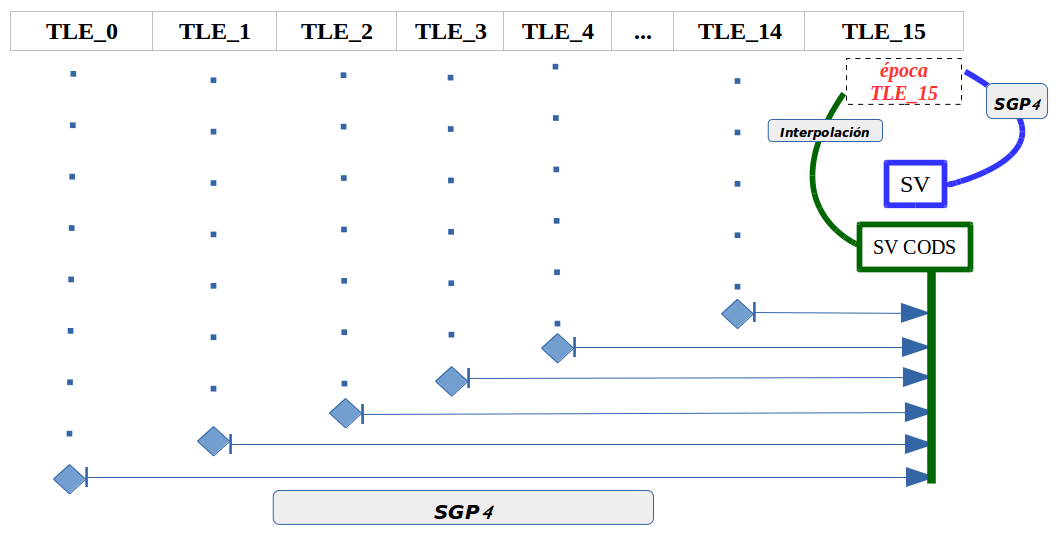
\includegraphics[width=0.7\textwidth]{imagenes/Osweiler_sobre_Cods.png}
 \caption{M\'etodo de Osweiler sobre datos CODS}
\end{figure}

\section{La Probabilidad de Colisi\'on}
{\bf{citar a Klinkrad}}
Dada la situaci\'on de encuentro, la PoC es el par\'ametro que se utiliza para delimitar m\'argenes operativos.
Es decir, que en base a ella se tomar\'an decisiones como realizar o no una maniobra.\\
Distintos autores han desarrollado varios m\'etodos para el c\'alculo de la PoC, y todos ellos comparten las siguientes consideraciones:\\
\begin{itemize}
 \item El error en la posici\'on puede representarse por una funci\'on de distribuci\'on Gaussiana 3D, cuya funci\'on de densidad de probabilidad se detalla en la eq...{\bf{bla}} 
 \item Tanto el objeto primario, como el desecho se mueven en movimiento rectil\'ineo con velocidad constante durante el encuentro.
 \item Los errores en las velocidades se desprecian.
 \item Los errores en las posiciones del objeto primario y del desecho no est\'an correlacionados.
 \item Los errores en las posiciones son constantes durante el encuentro, al igual que la matrices de covarianzas correspondientes al TCA.
\end{itemize}

\subsection*{M\'etodo de Akella}
En este trabajo para el c\'alculo de la PoC se utilizar\'a el m\'etodo de Alfriend \& Akella[4] ya que es conceptualmente simple y aunque tiene un alto costo computacional, es realizable por las m\'aquinas actuales en tiempos menores a un segundo.\\

El mismo requiere como entradas:
\begin{itemize}
 \item Conocer el instante de m\'aximo acercamiento: TCA (Time of Closest Approach).
 \item La posici\'on relativa del desecho respecto al objeto primario en el TCA.
 \item La velocidad relativa del desecho respecto al objeto primario en el TCA.
 \item Las matrices de error de ambos objetos.
\end{itemize}

En los momentos pr\'oximos al encuentro, la posici\'on relativa de riesgo $\Delta r$ puede expresarse en funci\'on de un intervalo de tiempo respecto del TCA, es decir, $\Delta t_{tca}=t-t_{tca}$.

\begin{equation}
 \Delta r(t)=\Delta r_{tca}+\Delta v_{tca}(t-t_{tca})
\end{equation}

Las matrices de covarianza de los errores que son calculadas para un momento dado t previo al TCA, deben ser propagadas. ({\bf{ver metodolog\'ia}})
Dado que consideramos que los errores en las posiciones de ambos objetos no est\'an correlacionadas, ambas contribuciones pueden combinarse en una \'unica matriz, a partir de la suma de ambas.

\begin{equation}
 C=C_{p}+C_{d}
\end{equation}

De $C$ s\'olo consideraremos la submatriz superior de la izquierda de dimensiones (3x3), que corresponde a los errores en las posiciones, con un $1 \sigma$.\\
Dado que adem\'as asumimos que los errores en la posici\'on son de distribuci\'on normal en 3D, la funci\'on densidad de probabilidad $p(\Delta r)$ en momentos pr\'oximos al m\'aximo acercamiento queda definida por la expresi\'on {\bf{eq ..bla}}:

\begin{equation}
 p(\Delta r)=\frac{1}{\sqrt((2 \pi)^3det(C))} exp[-\frac{1}{2}\Delta r^TC^{-1}\Delta r] 
\end{equation}



Sean $R_{t}$ y $R_{r}$ los radios de las esferas que encierran a nuestra misi\'on principal y al desecho de riesgo, respectivamente. Se considera una situaci\'on de {\it{encuentro}} o {\it{riesgo de colisi\'on}}, al hecho de que estas esferas se intersecten, o lo que es lo mismo, si ocurre un acercamiento dentro de una esfera de {\it{radio de colisi\'on}} $R_{c}$, secci\'on $A_{c}$,  volumen $V_{c}$.

\begin{equation}
R_{c}=R_{t}+R_{r} \qquad A_{c}=\pi R_{C}^{2} \qquad V_{c}=\frac{4}{3} \pi R_{c}^{3}
\end{equation}

La probabilidad de colisi\'on $P_{c}$ se calcula a partir de la integral de volumen de la funci\'on densidad de probabilidad (eq) sobre la regi\'on esf\'erica $V_{c}$, centrada en el desecho de riesgo.
\begin{equation}
PoC=\frac{1}{\sqrt((2\pi)^3det(C))} \int \limits_{Vc} exp[-\frac{1}{2}\Delta r^TC^{-1}\Delta r]dV
\label{eq:poc3d}
\end{equation}

Puede demostrarse que esta integral de volumen puede reducirse a una integral de superficie mapeando el elipsoide  de los errores en la posici\'on, en contornos el\'ipticos de probabilidad constante sobre el B-plane {\bf{(citar a Foster)}}.

El B-plane es perpendicular al vector velocidad relativa $\Delta v_{tca}$ en el momento de m\'aximo acercamiento.
A su vez, el vector $\Delta r_{tca}$ yace en el B-plane, como deja ver la ecuaci\'on de {\bf{zero-transit of the range-rate between the two objects}}:
\begin{equation}
 \frac{\Delta v_{tca} \Delta r_{tca}}{\Delta r_{tca}}= \dot{\rho}_{tca}=0.0 \quad \rightarrow \quad t_{tca}
\end{equation}

Definamos los vectores directores unitarios del plano como $X_{B}$ e $Y_{B}$, de acuerdo a las expresiones:

\begin{equation}
 X_{B}=\frac{\Delta r_{tca}}{|\Delta r_{tca}|} \quad Y_{B}=\frac{(\Delta r_{tca}) \times (\Delta v_{tca})}{|(\Delta r_{tca}) \times (\Delta v_{tca})|}
\end{equation}


A partir de estos vectores unitarios, se construye la matriz de transformaci\'on $R_{X_{B},Y_{B}}$ que mapea las matrices de covarianza en tres dimensiones $C=C_{x,y,z}$ a matrices de dos dimensiones en el B-plane $C_{B}$.

\begin{equation}
  C_{B} = C_{{X_{B},Y_{B}}} = R_{X_{B},Y_{B}} C R^{T}_{X_{B},Y_{B}}\\
\end{equation}

\begin{equation}
  R_{X_{B},Y_{B}} = 
  \begin{pmatrix}
    X_{B,X} & X_{B,Y} & X_{B,Z}\\
    Y_{B,X} & Y_{B,Y} & Y_{B,Z}
  \end{pmatrix}
\end{equation}

Los ejes principales de los contornos el\'ipticos de probabilidad constante, quedan determinados a partir de los autovalores $\lambda_{i,B}(i=1,2)$ y los autovectores $\bar{e}_{i,B}$ que resuelven la ecuaci\'on:

\begin{equation}
(C_{B} - \lambda_{i,B} I) \bar{e}_{i,B} = \bar{0}
\end{equation}

Donde $I$ es la matriz identidad $2x2$.

Ahora, sea la elipse que representa los errores de posici\'on de $1\sigma$ en el B-plane:\\

\begin{itemize}
 \item El {\bf{semieje mayor}} queda definido por: $a_{1\sigma,B}=\sqrt(max(\lambda_{1,B},\lambda_{2,B}))$
 \item El {\bf{semieje menor}} queda definido por: $b_{1\sigma,B}=\sqrt(min(\lambda_{1,B},\lambda_{2,B}))$
 \item La {\bf{direcci\'on del semieje mayor}} ser\'a $\bar{e}_{a,B}$, con vector unitario: $ \bar{x}_{B}=\frac{\bar{e}_{a,B}}{|\bar{e}_{a,B}|}$ 
 \item La {\bf{orientiaci\'on de $\bar{e}_{a,B}$}} respecto a la direcci\'on de la conjunci\'on $X_{B}$ la indica el \'angulo $\Phi_{B}$ (ver \ref{fig:bplane})
\end{itemize}

\begin{equation}
 \Phi_{B}= arccos(\bar{x}_{B},X_{B})
\end{equation}

\begin{figure}[!h]
\centering
 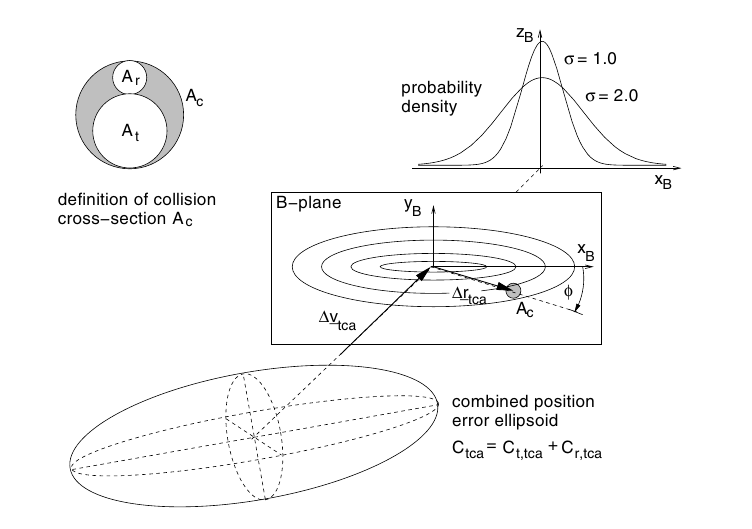
\includegraphics[width=0.5\textwidth]{imagenes/akellabplane}
 \caption{ B-plane (Adaptado de ....)}
 \label{fig:bplane}
\end{figure}

Bien, consideremos ahora una posici\'on relativa de acercamiento $\Delta r_{B}$ ya proyectada en el B-plane. La integral de volumen de la probabilidad de colisi\'on de la Eq. \ref{eq:poc3d} se reduce a una integral de superficie sobre la secci\'on circular de colisi\'on $R_{c}$, proyectada en el B-plane y centrada a la distancia relativa predicha en el instante de m\'aximo acercamiento, $\Delta r_{tca}$

\begin{equation}
P_{c} = \frac{1}{2 \pi \sqrt(det(C_{B}))} \int_{-R_{c}}^{+R_{c}} \int_{-\sqrt(R^{2}_{c}-x^{2}_{B})}^{+\sqrt(R^{2}_{c}-x^{2}_{B})} exp [- A_{B}] dy_{B} dx_{B}
\end{equation}

\begin{equation}
A_{B}=\frac{1}{2}\Delta r^{T}_{B} C^{-1}_{B} \Delta r_{B}
\end{equation}



\section{El CDM}
(JAC SW - Laporte)
{\bf{CSM:}} They are made available on Emergency Criteria, wich are Time of Closest Approach whithin 72 hs combined with a miss distance criteria:\\
LEO:\\
overall miss distance < 1km\\
radial miss distance < 200m\\
GEO/MEO:\\
Overall miss distance < 10 km.\\

CSM are advisory and informational messages only and are not directly actionable. They don´t provide a direct recommendation to perform an avoidance action and of course they cannot take neither the operational constraints of the asset nor the maneuvers the asset plansor just performed. (sigue ver apuntes Laporte carpeta...)\\

!!! JSpOC NO CUENTA CON INFORMACI\'ON DE MANIOBRAS PLANIFICADAS, puede haber falsas alarmas.\\




